\label{planificacion}

Una vez conocido el método de trabajo que se seguirá para el desarrollo del proyecto, se deben conocer los plazos en los cuales el proyecto debe ser finalizado y entregado.

La fecha de inicio del proyecto es, por tanto, \textit{el 15 de Octubre de 2019}, y la fecha límite en la cual el proyecto debe ser entregado data del \textit{29 de Febrero de 2020}.

\subsubsection{Disponibilidad del desarrollador}

El proyecto se debe ajustar a una extensión de 300 horas, como fué especificado en el cálculo de costes en el apartado \ref{duracion_proyecto} del presente documento.

En cuanto a la disponibilidad del proyecto, el desarrollador carece de suficiente tiempo  al día como para elaborar 8 horas díarias, asemejándose a un trabajo real, debido a tener que compaginar las 7 horas diarias de un trabajo externo, con las necesarias para la completitud de dos asignaturas de la Universidad, y el presente proyecto.

Tras una planificación semanal, el desarrollador es capaz de asignar una media de 24 horas semanales, lo que supondría poder finalizar el proyecto en:

\begin{center}
    \textit{24horas/semana / 6 dias laborables/semana = 4horas/dia }
    
    \textit{300horas / 4 horas/dia = 75 días }  

\end{center}

\newpage
\section{Diagramas de Gantt}

Al datarse de un proyecto basado en prototipos y dada la amplitud posible del mismo, se va a proceder a organizar el plan de trabajo en la secuencia del siguiente ciclo:
\begin{enumerate}
    \item \textit{Elicitación de requisitos} \newline
    Periodo en el cual se razona cuáles son los requisitos necesarios que se van a llevar a cabo en el protototipo a desarrollar. En es este periodo en el cual se realiza el diagrama de Gantt del prototipo indicado, planeando y estipulando los tiempos necesarios para llevar a cabo cada tarea.
    
    \item \textit{Desarrollo} \newline
    Esta etapa es en la cual se lleva a cabo la elaboración del prototipo siguiendo el plan de desarrollo estipulado en el punto anterior.
    
    \item \textit{Presentación del prototipo} \newline
    Reunión con el tutor para mostrar el prototipo y sus funcionalidades, con el fin de ver si se ha alcanzado lo esperado, al igual que para realizar un brainstorm conjunto con el fin de poder elicitar los requisitos del prototipo siguiente.
\end{enumerate}

La cuantía de prototipos elaborados será tanta como permitan las 300 horas de duración máxima del proyecto, enfocando cada prototipo en la completitud de un mínimo de requisitos con los cuales se busca un acercamiento a un prototipo final lo más aproximado posible a un producto final.

Debido a la condición del desarrollador que va a llevar a cabo el proyecto, se considera que cada día marcado en los siguientes diagramas corresponde con 4 horas de trabajo.

Para llevar a cabo la organización, se ha respetado un día libre a la semana, el cual coincide con el Domingo, al igual que se respetan los días festivos nacionales.

\textit{NOTA: Finalmente, tras la elaboración iterativa y ajuste de prototipos a las horas máximas marcadas se ha conseguido elaborar la cuantía de 4 prototipos, de los cuales se mostrarán sus diagramas de Gantt a continuación.}

\begin{sidewaysfigure}
\begin{figure}[H]
    \centering
    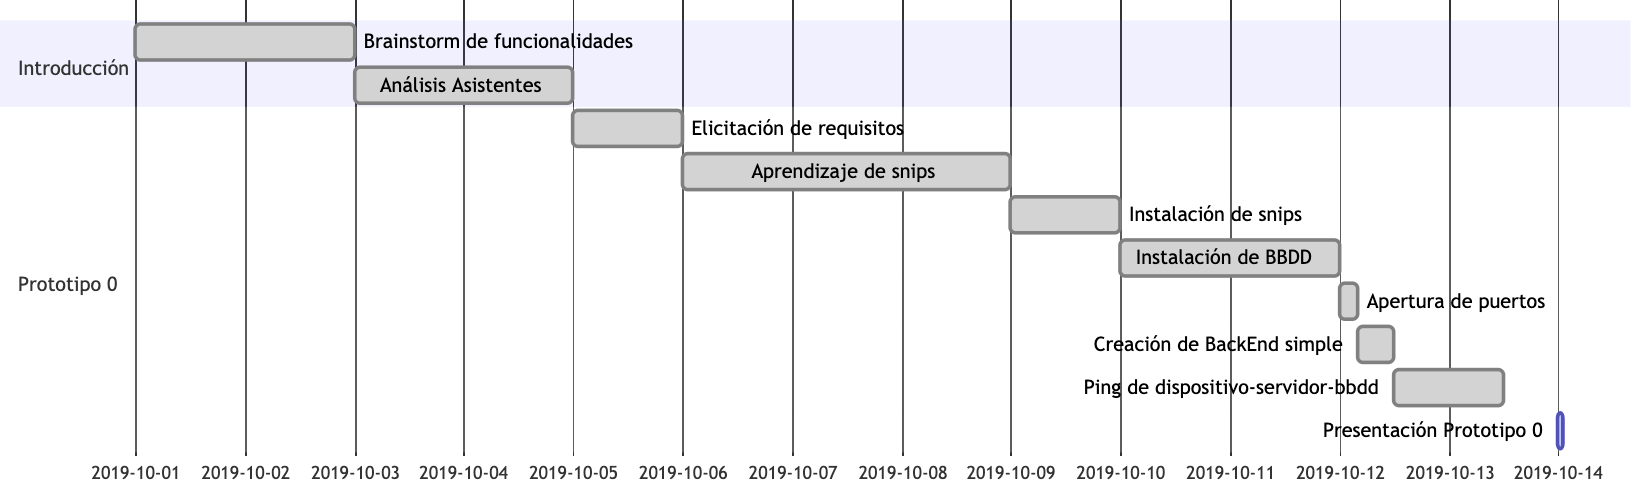
\includegraphics[width=19cm]{./img/grantt/p0.png}
    \caption{Diagrama de Gantt - Prototipo 0}
    \label{fig:grant.p0}
\end{figure}
\end{sidewaysfigure}

\begin{sidewaysfigure}
\begin{figure}[H]
    \centering
    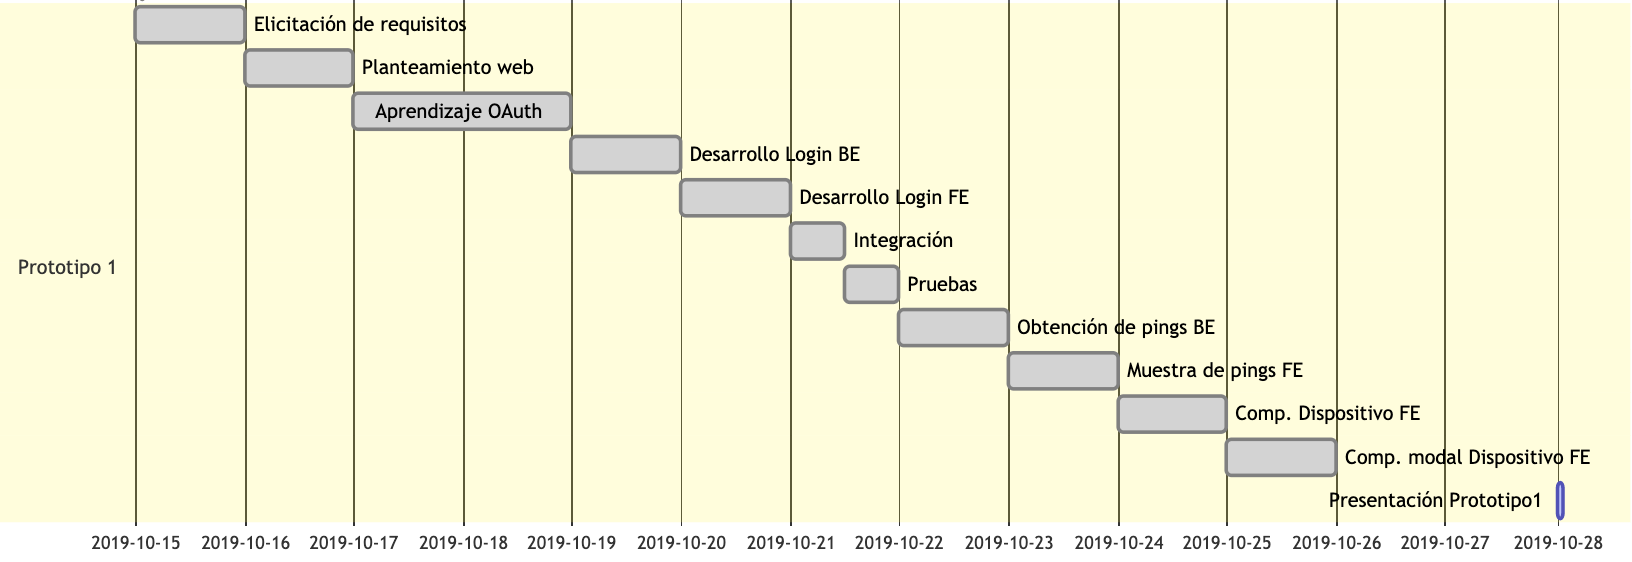
\includegraphics[width=19cm]{./img/grantt/p1.png}
    \caption{Diagrama de Gantt - Prototipo 1}
    \label{fig:grant.p1}
\end{figure}
\end{sidewaysfigure}

\begin{sidewaysfigure}
\begin{figure}[H]
    \centering
    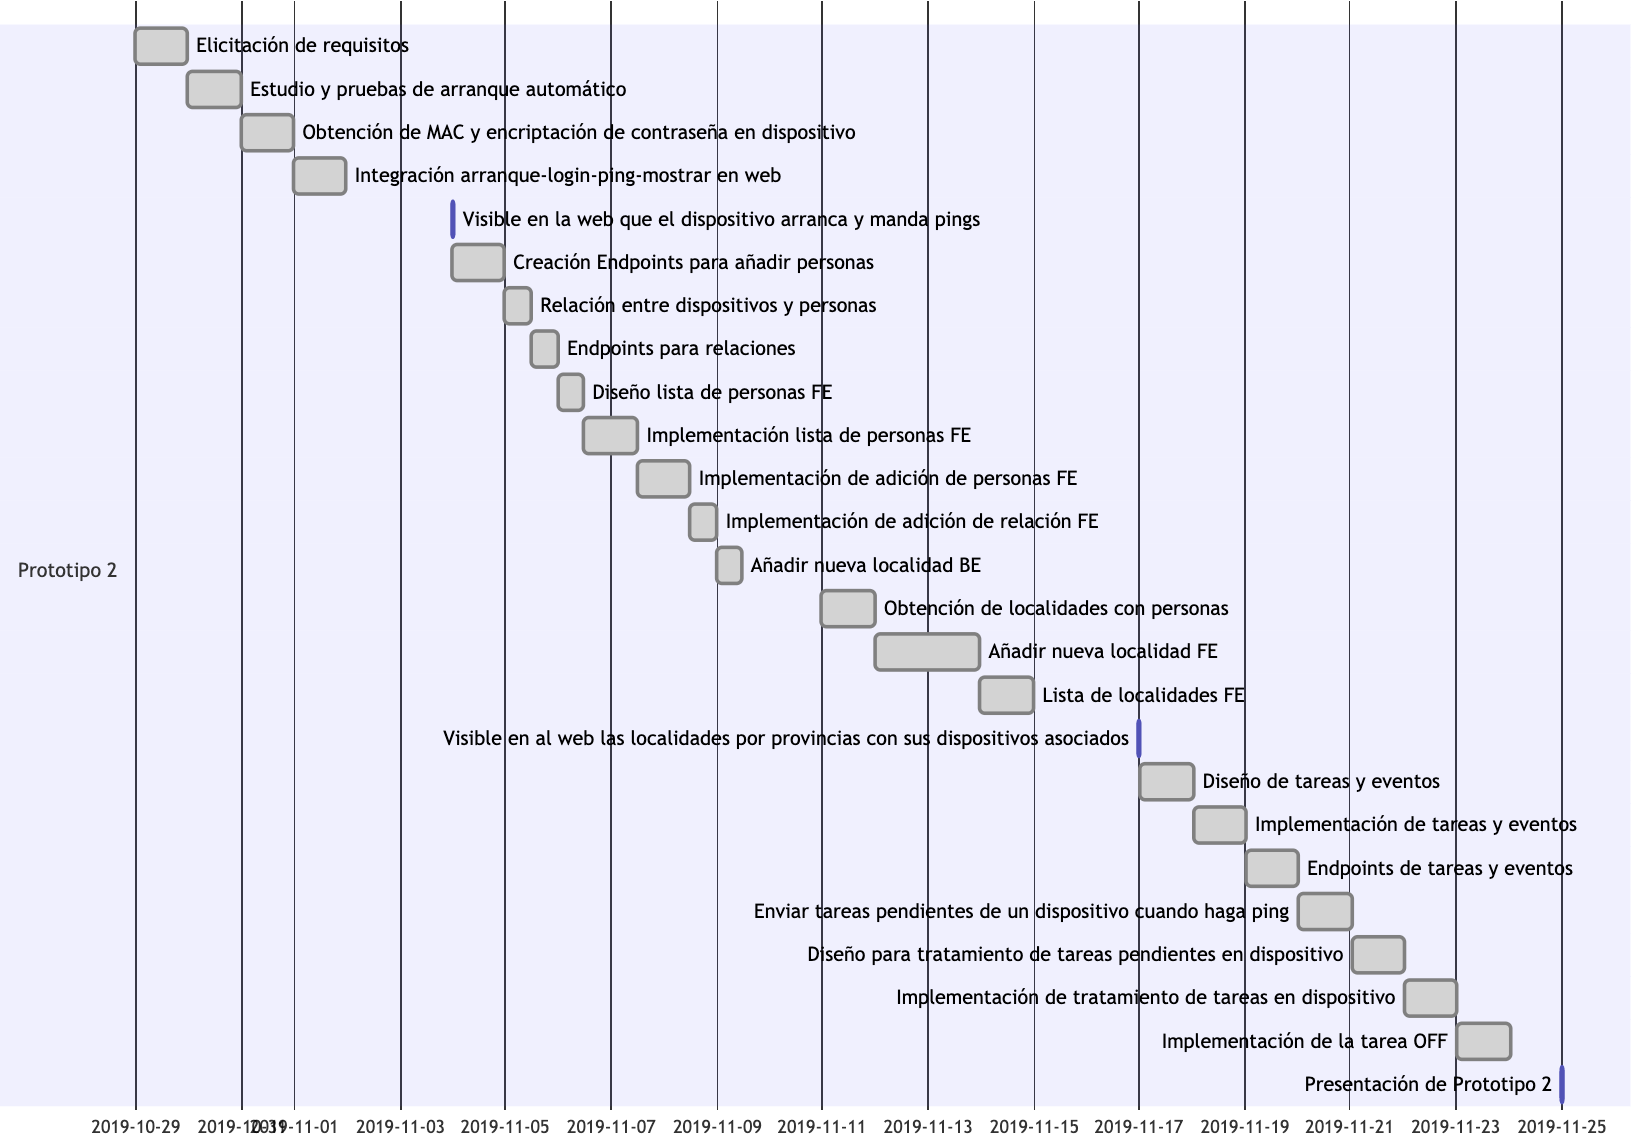
\includegraphics[width=19cm]{./img/grantt/p2.png}
    \caption{Diagrama de Gantt - Prototipo 2}
    \label{fig:grant.p2}
\end{figure}
\end{sidewaysfigure}

\begin{sidewaysfigure}
\begin{figure}[H]
    \centering
    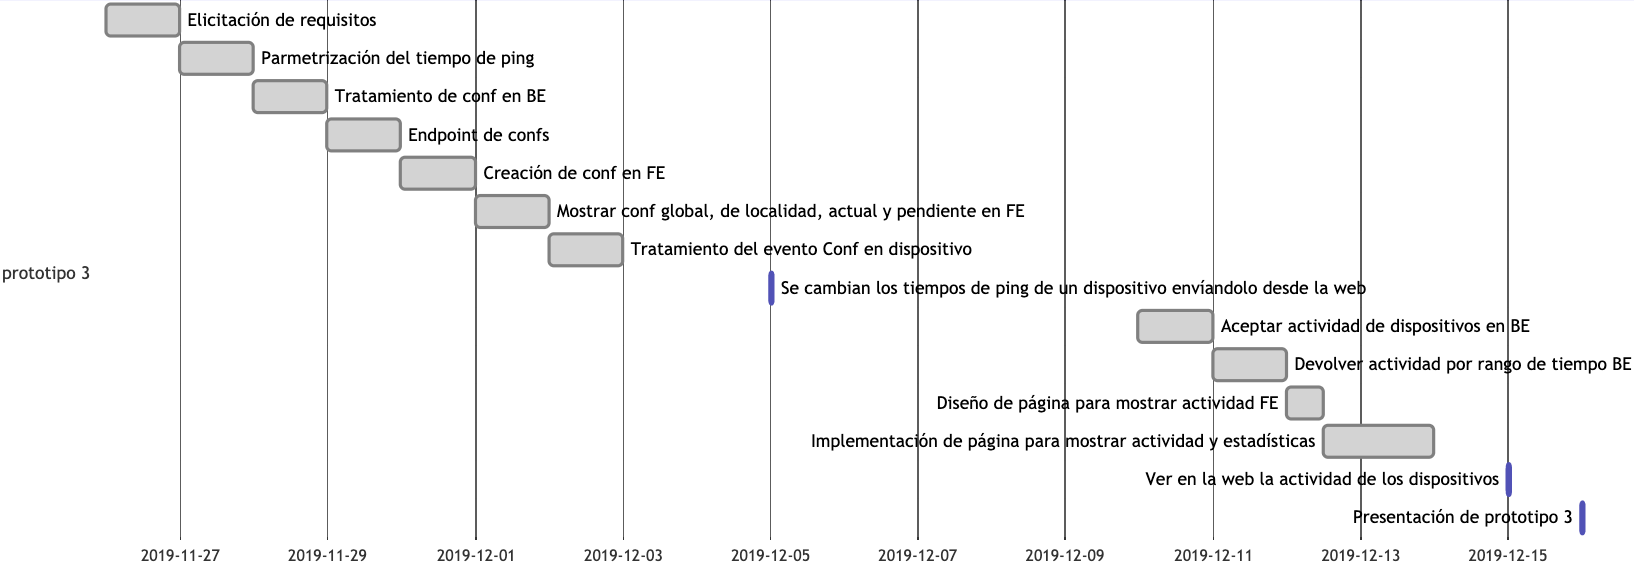
\includegraphics[width=19cm]{./img/grantt/p3.png}
    \caption{Diagrama de Gantt - Prototipo 3}
    \label{fig:grant.p3}
\end{figure}
\end{sidewaysfigure}

\begin{sidewaysfigure}
\begin{figure}[H]
    \centering
    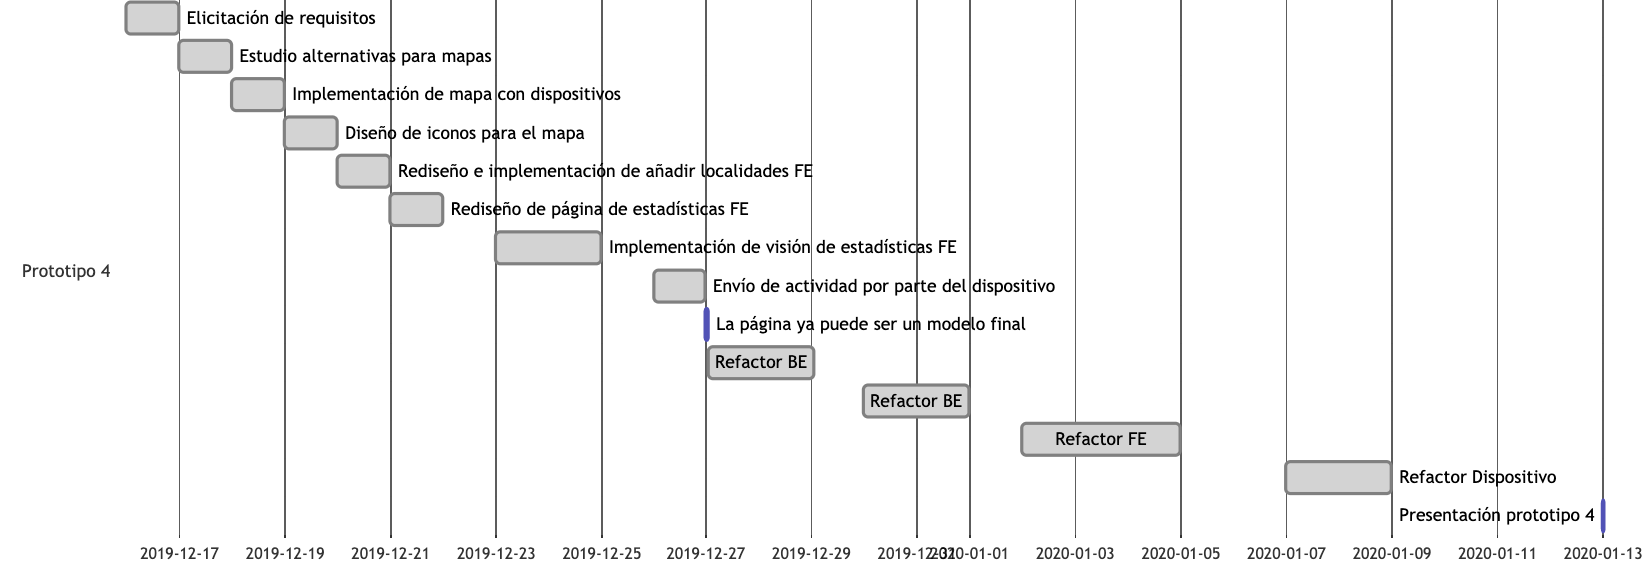
\includegraphics[width=19cm]{./img/grantt/p4.png}
    \caption{Diagrama de Gantt: Prototipo 4}
    \label{fig:grant.p3s}
\end{figure}
\end{sidewaysfigure}